\documentclass[10pt,a4paper]{article}

\usepackage[a4paper,margin=1.6cm,top=1.8cm,bottom=1.8cm]{geometry}
\usepackage{microtype}
\usepackage{xcolor}
\usepackage{booktabs,array,tabularx,enumitem,multicol,adjustbox}
\usepackage{listings}
\usepackage{tikz}
\usetikzlibrary{arrows.meta,positioning,shapes.multipart,fit,backgrounds,calc}
\usepackage{fancyhdr}
\usepackage[hidelinks]{hyperref}

\definecolor{soft}{gray}{0.92}
\definecolor{mid}{gray}{0.55}

\setcounter{secnumdepth}{0}
\Urlmuskip=0mu plus 1mu
\setlength{\emergencystretch}{3em}
\setlength{\parindent}{0pt}
\setlength{\parskip}{3pt}
\setlist{nosep,leftmargin=1.2em}
\renewcommand{\arraystretch}{1.15}

\pagestyle{fancy}
\fancyhf{}
\fancyhead[L]{\small ELE-IWS-521 \textbar{} React + Full-Stack Blog Cheat Sheet}
\fancyfoot[C]{\small\thepage}
\renewcommand{\headrulewidth}{0.4pt}

% ---------- headings (plain, black and white) ----------
\makeatletter
\renewcommand\section{\@startsection{section}{1}{\z@}{1.2em plus .3em}{.5em}{\large\bfseries\scshape}}
\renewcommand\subsection{\@startsection{subsection}{2}{\z@}{.9em plus .2em}{.3em}{\normalsize\bfseries}}
\makeatother

% ---------- code listings ----------
\lstdefinelanguage{JS}{
  keywords={const,let,var,function,return,if,else,async,await,import,export,from,default,try,catch,finally,new,throw,for,of,in,true,false,null,undefined,class,extends},
  sensitive=true, comment=[l]{//}, morecomment=[s]{/*}{*/},
  morestring=[b]', morestring=[b]", morestring=[b]`
}
\lstset{
  basicstyle=\ttfamily\footnotesize, keywordstyle=\bfseries, commentstyle=\itshape\color{mid},
  stringstyle=\color{black!70}, frame=single, rulecolor=\color{mid}, backgroundcolor=\color{soft},
  breaklines=true, columns=fullflexible, keepspaces=true, xleftmargin=2pt, xrightmargin=2pt,
  aboveskip=4pt, belowskip=2pt, showstringspaces=false, tabsize=2
}
\lstdefinestyle{sql}{language=SQL, keywordstyle=\bfseries, morekeywords={returning,conflict,nothing,unnest,ilike,limit,offset,trigger,function,plpgsql}}

\newcommand{\code}[1]{\texttt{#1}}

% ---------- TikZ styles ----------
\tikzset{
  box/.style={draw, rounded corners=2pt, align=center, minimum height=7mm, inner sep=3pt, font=\footnotesize, fill=white},
  soft/.style={box, fill=soft},
  dark/.style={box, fill=black, text=white},
  arr/.style={-{Stealth[length=2.2mm]}, thick},
  darr/.style={-{Stealth[length=2.2mm]}, thick, dashed},
  lab/.style={font=\scriptsize, fill=white, inner sep=1pt},
  zone/.style={draw, dashed, rounded corners=4pt, inner sep=6pt}
}

\begin{document}

\begin{center}
{\LARGE\bfseries React + Full-Stack Blog Cheat Sheet}\\[2pt]
{\large Learn React, and see how our whole system fits together}\\[2pt]
\small ELE-IWS-521 \textbar{} React frontend $\cdot$ Express API $\cdot$ PostgreSQL on Supabase
\end{center}

\begin{tabularx}{\linewidth}{@{}X@{}}
\toprule
\textbf{How to use this sheet.} Part A teaches the React ideas you will be asked about (components, props, state, the virtual DOM, hooks, routing).
Part B draws our project: architecture, request flow, login flow, database, component tree. Part C is quick reference (endpoints, SQL, Git).
Every example here comes from our own code, so open the file named in the text and read it next to the sheet. \\
\bottomrule
\end{tabularx}

% =====================================================================
\section{Part A --- React in one sitting}

\subsection{A1. The one big idea: UI = function of state}
You do \textbf{not} tell the browser how to change the page. You describe what the page should look like for the current data (\emph{state}); React works out the changes.
When state changes React does three things: \textbf{render} (call your component again), \textbf{diff} (compare the new description with the old one), \textbf{commit} (touch only the real DOM nodes that differ).

\begin{center}
\adjustbox{max width=\linewidth}{%
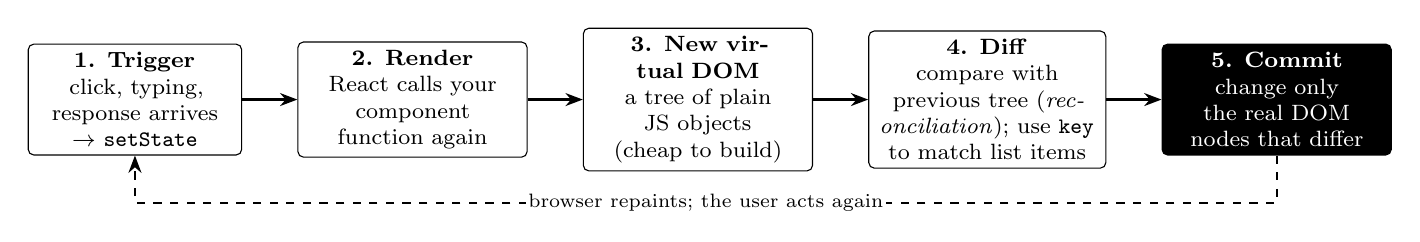
\begin{tikzpicture}[node distance=7mm]
  \node[box, text width=2.5cm] (s) {\textbf{1. Trigger}\\ click, typing, response arrives $\rightarrow$ \code{setState}};
  \node[box, text width=2.7cm, right=of s] (r) {\textbf{2. Render}\\ React calls your component function again};
  \node[box, text width=2.7cm, right=of r] (v) {\textbf{3. New virtual DOM}\\ a tree of plain JS objects (cheap to build)};
  \node[box, text width=2.8cm, right=of v] (d) {\textbf{4. Diff}\\ compare with previous tree (\emph{reconciliation}); use \code{key} to match list items};
  \node[dark, text width=2.7cm, right=of d] (c) {\textbf{5. Commit}\\ change only the real DOM nodes that differ};
  \draw[arr] (s) -- (r); \draw[arr] (r) -- (v); \draw[arr] (v) -- (d); \draw[arr] (d) -- (c);
  \draw[darr] (c.south) -- ++(0,-6mm) -| node[lab, pos=.25] {browser repaints; the user acts again} (s.south);
\end{tikzpicture}}
\end{center}

\subsection{A2. JSX is just function calls}
\begin{minipage}[t]{0.49\linewidth}
\begin{lstlisting}[language=JS]
// What you write (JSX)
<button className="btn" onClick={save}>
  Save {count}
</button>
\end{lstlisting}
\end{minipage}\hfill
\begin{minipage}[t]{0.49\linewidth}
\begin{lstlisting}[language=JS]
// What it becomes
jsx("button", {
  className: "btn", onClick: save,
  children: ["Save ", count],
})
// which returns a plain object:
// { type: "button", props: {...} }
\end{lstlisting}
\end{minipage}

Rules: one root element (or \code{<>...</>}); \code{className} not \code{class}; \code{\{ \}} embeds any JavaScript \emph{expression}; every tag must close (\code{<img />}).
Components start with a \textbf{capital letter} so React can tell \code{<Navbar />} from \code{<nav>}.

\subsection{A3. Components, props, and one-way data flow}
A component is a function that takes \textbf{props} (inputs, read-only) and returns JSX. Data flows \textbf{down} through props; events flow \textbf{up} by calling a function the parent passed in.
That makes bugs easy to trace: to find who changed the data, look \emph{up} the tree.

\begin{center}
\adjustbox{max width=0.8\linewidth}{%
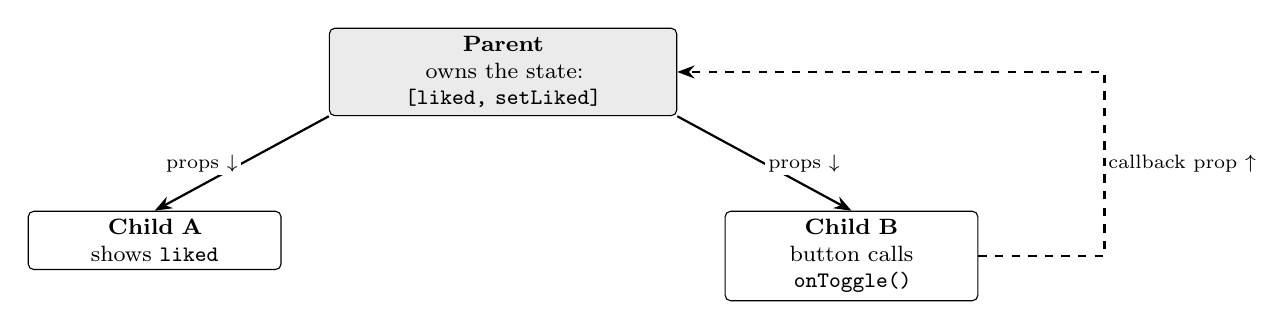
\begin{tikzpicture}[node distance=10mm]
  \node[soft, text width=4.2cm] (p) {\textbf{Parent}\\ owns the state: \code{[liked, setLiked]}};
  \node[box, text width=3cm, below left=12mm and 6mm of p] (a) {\textbf{Child A}\\ shows \code{liked}};
  \node[box, text width=3cm, below right=12mm and 6mm of p] (b) {\textbf{Child B}\\ button calls \code{onToggle()}};
  \draw[arr] (p.south west) -- node[lab, pos=.5, left] {props $\downarrow$} (a.north);
  \draw[arr] (p.south east) -- node[lab, pos=.5, right] {props $\downarrow$} (b.north);
  \draw[darr] (b.east) -- ++(1.6,0) |- node[lab, pos=.25, right] {callback prop $\uparrow$} (p.east);
\end{tikzpicture}}
\end{center}

\begin{lstlisting}[language=JS]
function PostCard({ post, onDelete }) {          // props arrive as one object; we destructure it
  return (
    <article>
      <h2>{post.title}</h2>
      {post.status === "draft" && <span>Draft</span>}      {/* conditional rendering */}
      <button onClick={() => onDelete(post.id)}>Delete</button>   {/* event goes UP via a callback */}
    </article>
  );
}
{posts.map((p) => <PostCard key={p.id} post={p} onDelete={remove} />)}   // key = stable id, NOT the array index
\end{lstlisting}

\subsection{A4. State: a component's memory}
\begin{multicols}{2}
\begin{lstlisting}[language=JS]
const [count, setCount] = useState(0);

setCount(count + 1);            // ok
setCount((c) => c + 1);         // best when the new
                                // value depends on the old
// NEVER mutate state:
items.push(x); setItems(items); // wrong
setItems([...items, x]);        // right (new array)
setUser({ ...user, name: "Ann" });   // new object
\end{lstlisting}
\columnbreak
\begin{itemize}
  \item State is a \textbf{snapshot}: inside one render, \code{count} never changes, even after \code{setCount}.
  \item Calling \code{setState} \textbf{schedules} a re-render; it does not change the variable you already hold.
  \item \textbf{Controlled input}: \code{value} comes from state, \code{onChange} writes back to state. React is the single source of truth.
  \item Keep state \textbf{as low as possible}; lift it up only to the nearest parent that needs to share it.
  \item Don't store what you can compute (e.g.\ \code{totalPages} from \code{total} and \code{limit}).
\end{itemize}
\end{multicols}

\subsection{A5. Hooks}
Hooks are functions starting with \code{use} that let a component remember things and react to the outside world. \textbf{Rules:} call them at the top level of a component (never inside \code{if}, loops or callbacks), and only from components or other hooks.

\begin{tabularx}{\linewidth}{@{}>{\ttfamily}l X@{}}
\toprule
\textbf{Hook} & \textbf{Use it for (and where we use it)} \\ \midrule
useState & Local values that change: form fields, open/closed, loaded data (Login form, Editor). \\
useEffect & Sync with something outside React: fetch data, timers, event listeners. Runs \emph{after} render; re-runs when a dependency changes; the returned function is cleanup (\code{useFetch}, \code{useDebounce}). \\
useContext & Read shared data without passing props through every level (\code{useAuth()} reads \code{AuthContext}: user, login, logout). \\
useRef & A box that survives renders and does \emph{not} trigger one: DOM nodes, timers, flags (\code{busy} in \code{LikeButton}). \\
useMemo / useCallback & Cache a calculation or a function between renders. Only when measured slowness or a memoised child needs it (\code{MarkdownView} memoises sanitised HTML). \\
useReducer & State with many related transitions; like \code{useState} with named actions. We did not need it. \\
\bottomrule
\end{tabularx}

\textbf{Dependency array:} \code{[]} run once after mount; \code{[a,b]} run when \code{a} or \code{b} change; no array = after every render (usually a bug).

\textbf{Our own custom hook} (\code{hooks/useDebounce.js}) --- a custom hook is just a function that uses other hooks:
\begin{lstlisting}[language=JS]
export default function useDebounce(value, delay = 400) {
  const [debounced, setDebounced] = useState(value);       // 1. remember a delayed copy of the value
  useEffect(() => {
    const timer = setTimeout(() => setDebounced(value), delay);   // 2. after `delay` ms with no change, copy it
    return () => clearTimeout(timer);       // 3. cleanup: value changed again, cancel the old timer
  }, [value, delay]);                       // 4. restart whenever value or delay changes
  return debounced;                         // 5. the search box calls the API with this, not every keystroke
}
\end{lstlisting}

\subsection{A6. Fetching data with effects}
\begin{lstlisting}[language=JS]
useEffect(() => {
  let cancelled = false;                    // ignore a late response if we already moved on (stale update bug)
  setLoading(true);
  api.get(`/posts?page=${page}`)
    .then((data) => { if (!cancelled) { setData(data); setLoading(false); } })
    .catch((err)  => { if (!cancelled) { setError(err); setLoading(false); } });
  return () => { cancelled = true; };       // cleanup
}, [page]);                                  // re-fetch when the page changes
\end{lstlisting}
Every data screen needs \textbf{three states}: loading, error (with a retry), and empty. We wrapped this pattern in \code{useFetch}. Don't use an effect for things you can calculate during render or do inside an event handler
(\href{https://react.dev/learn/you-might-not-need-an-effect}{\emph{You Might Not Need an Effect}}).

\subsection{A7. Routing, and client-side vs server-side rendering}
\begin{multicols}{2}
\begin{lstlisting}[language=JS]
<Routes>
  <Route element={<Layout />}>   {/* Navbar + <Outlet/> */}
    <Route index element={<Feed />} />
    <Route path="post/:id" element={<PostPage />} />
    <Route element={<ProtectedRoute roles={["admin"]} />}>
      <Route path="admin" element={<Admin />} />
    </Route>
    <Route path="*" element={<NotFound />} />
  </Route>
</Routes>

const { id } = useParams();           // /post/7 -> "7"
const navigate = useNavigate();       // navigate("/login")
const [params, setParams] = useSearchParams();  // ?q=maize
\end{lstlisting}
\columnbreak
\begin{itemize}
  \item \code{<Link>} / \code{<NavLink>} change the URL \emph{without} a page reload; plain \code{<a>} reloads.
  \item \code{<Outlet />} is where the matching child route renders.
  \item \textbf{URL as state:} we keep \code{page}, \code{q}, \code{tag} in the URL so links can be shared and Back works.
  \item \code{ProtectedRoute} redirects visitors who are not allowed. It is a \emph{convenience}: the API still checks every request.
  \item \code{React.lazy} + \code{Suspense} download rarely used pages only when opened (saves data).
\end{itemize}
\end{multicols}

\begin{tabularx}{\linewidth}{@{}>{\bfseries}l X X@{}}
\toprule
 & \textbf{Client-side rendering (our app)} & \textbf{Server-side rendering (e.g.\ Next.js)} \\ \midrule
First load & Browser gets a near-empty HTML file, then downloads JS, then fetches data and draws. & Server sends finished HTML; JS then ``hydrates'' it. \\
Search engines / link previews & May see an empty page unless pre-rendered. & See full content. \\
After first load & Very fast navigation, only JSON travels. & Also fast, plus extra server work. \\
Hosting & Static files (Vercel) + separate API. & Needs a server runtime. \\
\bottomrule
\end{tabularx}

\subsection{A8. Where should state live? (our choices)}
\begin{tabularx}{\linewidth}{@{}>{\bfseries}l X X@{}}
\toprule
\textbf{Kind of state} & \textbf{Where} & \textbf{Why} \\ \midrule
Form fields, open/closed & \code{useState} in the component & Only that component cares. \\
Logged-in user, token & \code{AuthContext} (Context API) & Many distant components need it; changes rarely. \\
Page, search text, tag & URL (\code{useSearchParams}) & Shareable, survives refresh, Back button works. \\
Server data (posts, comments) & \code{useFetch} + local state & Small app; a cache library (TanStack Query) or Redux would be extra weight. \\
Unsaved draft & \code{localStorage} via \code{useAutosaveDraft} & Must survive refresh or a dropped connection. \\
\bottomrule
\end{tabularx}

\subsection{A9. Optimistic update (likes and comments)}
Show the result \emph{now}, confirm with the server \emph{after}, undo if it failed. Source: \code{components/LikeButton.jsx}.
\begin{lstlisting}[language=JS]
const previous = like;                                   // 1. remember how things were
setLike({ liked: !previous.liked, count: previous.count + (previous.liked ? -1 : 1) });   // 2. update the UI immediately
try {
  const res = previous.liked ? await api.del(url) : await api.post(url);
  setLike({ liked: res.liked, count: res.likeCount });   // 3. the server's answer is the truth
} catch {
  setLike(previous);                                     // 4. rollback
  setError("Could not save your like.");                 // 5. tell the user
}
\end{lstlisting}

\subsection{A10. Bugs you will meet (and the fix)}
\begin{tabularx}{\linewidth}{@{}X X@{}}
\toprule
\textbf{Symptom} & \textbf{Usual cause $\rightarrow$ fix} \\ \midrule
Warning: each child needs a unique \code{key} & Missing \code{key} in \code{.map()} $\rightarrow$ use the item's database id. \\
Screen doesn't update after \code{setState} & You mutated the old array/object $\rightarrow$ create a new one (\code{[...a, x]}, \code{\{...o, k: v\}}). \\
Infinite loop of requests & \code{useEffect} sets state it also depends on, or has no dependency array $\rightarrow$ fix the array. \\
Old value inside a callback (stale closure) & Closure captured an old render $\rightarrow$ use the functional update \code{setX(x => ...)} or add the dependency. \\
Shows \code{[object Object]} or crashes & Rendering an object $\rightarrow$ render its fields. \\
Data arrives for a page you already left & Missing cleanup $\rightarrow$ the \code{cancelled} flag or \code{AbortController}. \\
Typing in an input does nothing & Controlled input without \code{onChange} $\rightarrow$ add \code{onChange} that sets state. \\
Works in dev, 404 on refresh in production & SPA needs a rewrite to \code{index.html} $\rightarrow$ \code{vercel.json}. \\
\bottomrule
\end{tabularx}

\subsection{A11. Two-week study path}
\begin{tabularx}{\linewidth}{@{}>{\bfseries}l X@{}}
\toprule
Days 1--3 & react.dev \emph{Learn}: Describing the UI (JSX, props, conditional rendering, lists, keeping components pure). \\
Days 4--6 & Adding Interactivity: events, state, \emph{Render and Commit}, state as a snapshot, updating objects and arrays. \\
Days 7--9 & Managing State and Escape Hatches: sharing state, \emph{Preserving and Resetting State} (keys), Context, refs, effects. \\
Days 10--12 & \emph{Reusing Logic with Custom Hooks}. Read our hooks and components; change one thing per file and watch what breaks. \\
Days 13--14 & Rehearse: explain one component and one hook out loud, line by line, without notes. \\
\bottomrule
\end{tabularx}

% =====================================================================
\newpage
\section{Part B --- Our project's architecture}

\subsection{B1. System architecture}
\begin{center}
\adjustbox{max width=\linewidth}{%
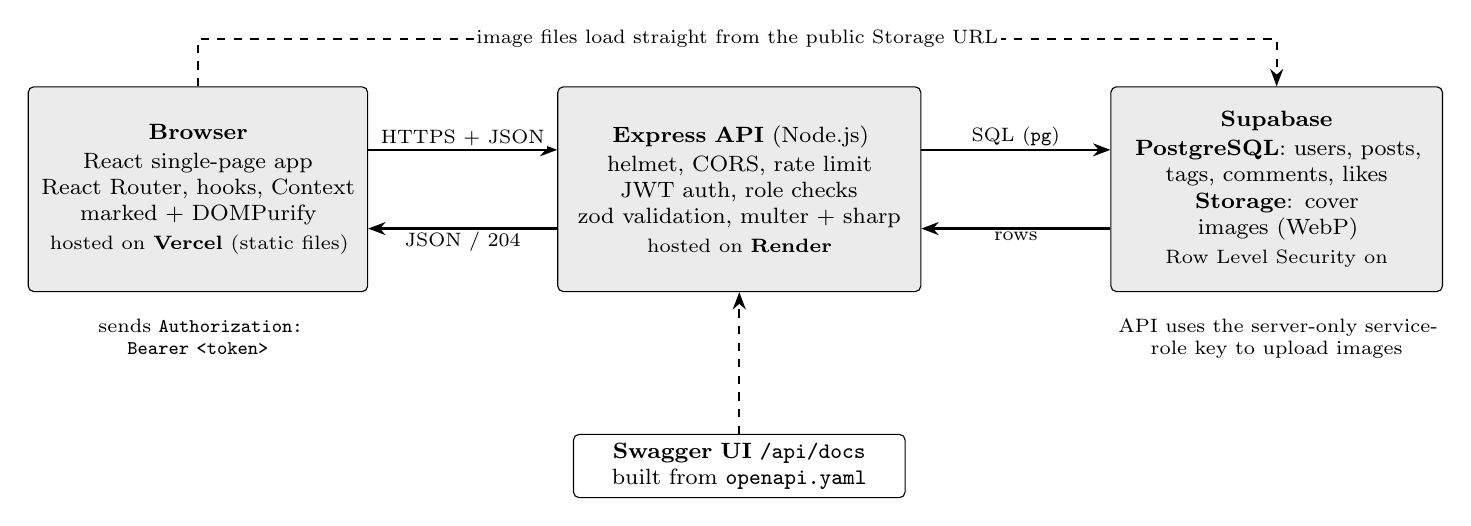
\begin{tikzpicture}[node distance=24mm]
  \node[soft, text width=4.1cm, minimum height=2.6cm] (web) {\textbf{Browser}\\[1pt] React single-page app\\ React Router, hooks, Context\\ marked + DOMPurify\\[1pt]\scriptsize hosted on \textbf{Vercel} (static files)};
  \node[soft, text width=4.4cm, minimum height=2.6cm, right=of web] (api) {\textbf{Express API} (Node.js)\\[1pt] helmet, CORS, rate limit\\ JWT auth, role checks\\ zod validation, multer + sharp\\[1pt]\scriptsize hosted on \textbf{Render}};
  \node[soft, text width=4cm, minimum height=2.6cm, right=of api] (db) {\textbf{Supabase}\\[1pt] \textbf{PostgreSQL}: users, posts, tags, comments, likes\\ \textbf{Storage}: cover images (WebP)\\[1pt]\scriptsize Row Level Security on};
  \draw[arr] ([yshift=5mm]web.east) -- node[lab, above] {HTTPS + JSON} ([yshift=5mm]api.west);
  \draw[arr] ([yshift=-5mm]api.west) -- node[lab, below] {JSON / 204} ([yshift=-5mm]web.east);
  \draw[arr] ([yshift=5mm]api.east) -- node[lab, above] {SQL (\code{pg})} ([yshift=5mm]db.west);
  \draw[arr] ([yshift=-5mm]db.west) -- node[lab, below] {rows} ([yshift=-5mm]api.east);
  \node[lab, below=3mm of web, text width=4cm, align=center] {sends \code{Authorization: Bearer <token>}};
  \node[lab, below=3mm of db, text width=4cm, align=center] {API uses the server-only service-role key to upload images};
  \draw[darr] (web.north) -- ++(0,6mm) -| node[lab, pos=.25] {image files load straight from the public Storage URL} (db.north);
  \node[box, below=18mm of api, text width=4cm] (sw) {\textbf{Swagger UI} \code{/api/docs}\\ built from \code{openapi.yaml}};
  \draw[darr] (sw) -- (api);
\end{tikzpicture}}
\end{center}

\subsection{B2. What happens to one API request (middleware pipeline)}
\begin{center}
\adjustbox{max width=\linewidth}{%
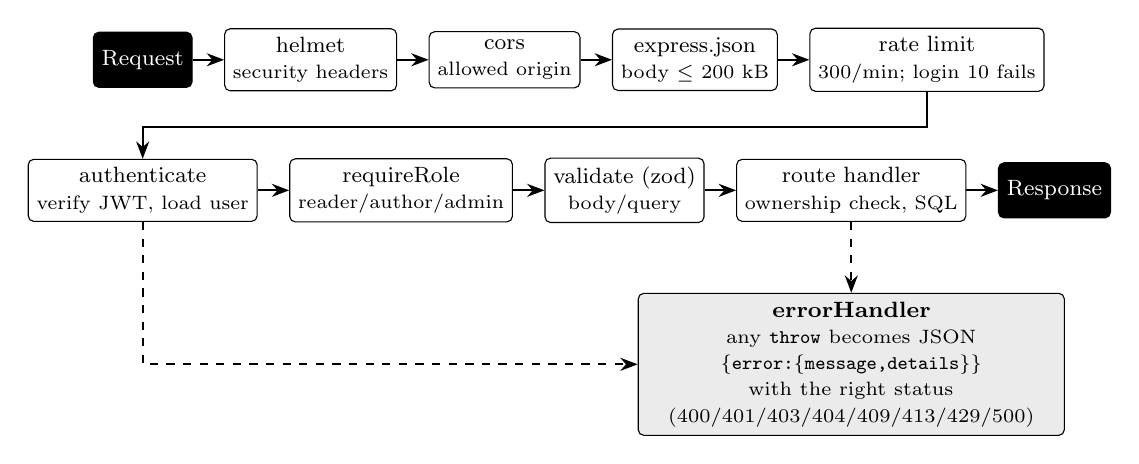
\begin{tikzpicture}[node distance=4mm]
  \node[dark] (req) {Request};
  \node[box, right=of req] (h) {helmet\\\scriptsize security headers};
  \node[box, right=of h] (c) {cors\\\scriptsize allowed origin};
  \node[box, right=of c] (j) {express.json\\\scriptsize body $\le$ 200 kB};
  \node[box, right=of j] (r) {rate limit\\\scriptsize 300/min; login 10 fails};
  \node[box, below=9mm of req, xshift=0mm] (a) {authenticate\\\scriptsize verify JWT, load user};
  \node[box, right=of a] (rr) {requireRole\\\scriptsize reader/author/admin};
  \node[box, right=of rr] (v) {validate (zod)\\\scriptsize body/query};
  \node[box, right=of v] (hd) {route handler\\\scriptsize ownership check, SQL};
  \node[dark, right=of hd] (res) {Response};
  \draw[arr] (req) -- (h); \draw[arr] (h) -- (c); \draw[arr] (c) -- (j); \draw[arr] (j) -- (r);
  \draw[arr] (r.south) -- ++(0,-4.5mm) -| (a.north);
  \draw[arr] (a) -- (rr); \draw[arr] (rr) -- (v); \draw[arr] (v) -- (hd); \draw[arr] (hd) -- (res);
  \node[soft, below=9mm of hd, text width=5.2cm] (err) {\textbf{errorHandler}\\\scriptsize any \code{throw} becomes JSON \code{\{error:\{message,details\}\}} with the right status (400/401/403/404/409/413/429/500)};
  \draw[darr] (a.south) |- (err.west);
  \draw[darr] (hd.south) -- (err.north);
\end{tikzpicture}}
\end{center}
Failing a step stops the chain: no token $\rightarrow$ \textbf{401}; wrong role or not the owner $\rightarrow$ \textbf{403}; bad input $\rightarrow$ \textbf{400} with field messages; missing/hidden resource $\rightarrow$ \textbf{404}.

\subsection{B3. Login, token, and a protected request}
\begin{center}
\adjustbox{max width=\linewidth,max totalheight=9.2cm}{%
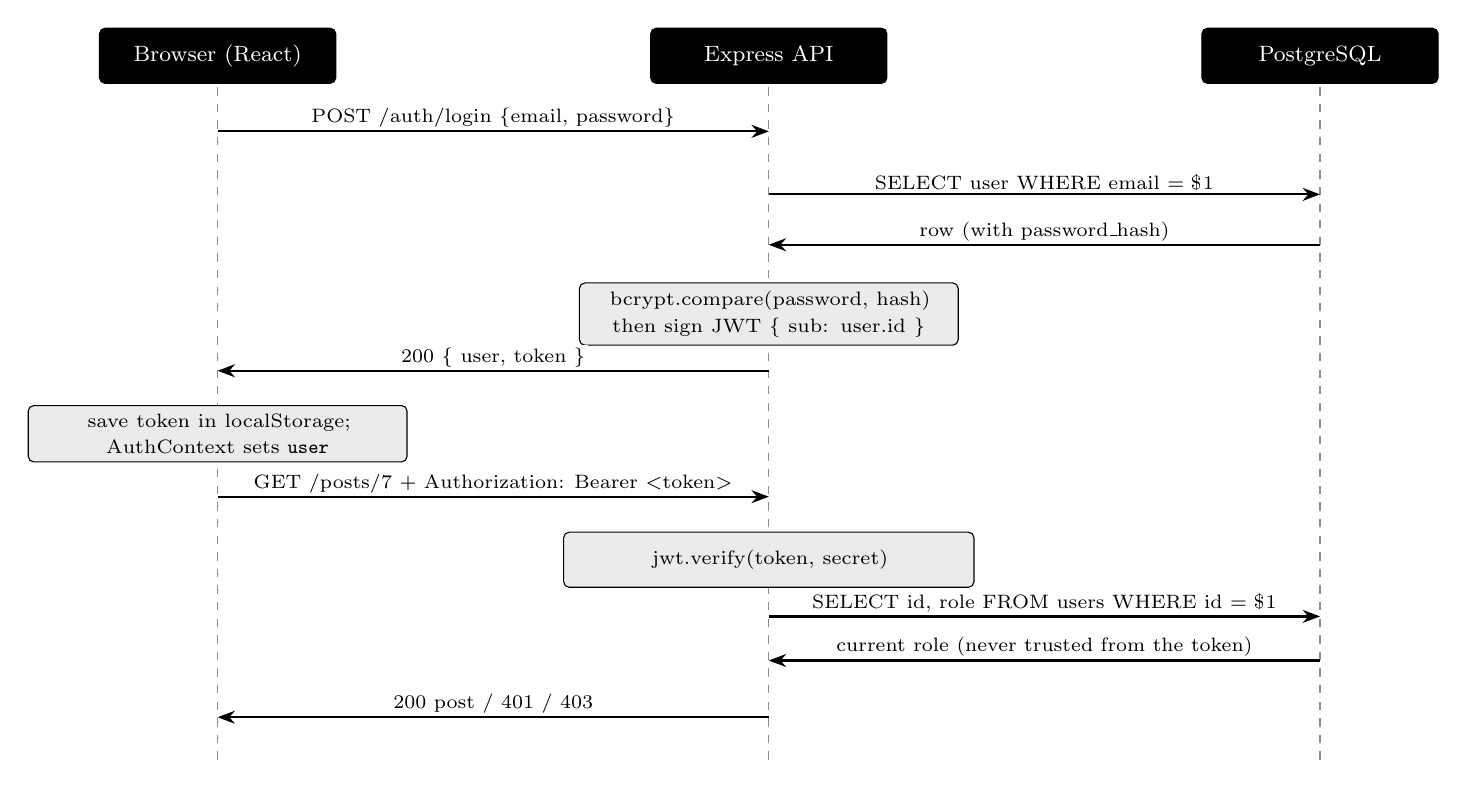
\begin{tikzpicture}[x=1cm,y=0.8cm]
  \foreach \x/\n in {0/Browser (React), 7/Express API, 14/PostgreSQL} {
    \node[dark, minimum width=3cm] (h\x) at (\x,0) {\n};
    \draw[mid, dashed] (\x,-0.5) -- (\x,-11.2);
  }
  \draw[arr] (0,-1.2) -- node[lab, above] {POST /auth/login \{email, password\}} (7,-1.2);
  \draw[arr] (7,-2.2) -- node[lab, above] {SELECT user WHERE email = \$1} (14,-2.2);
  \draw[arr] (14,-3.0) -- node[lab, above] {row (with password\_hash)} (7,-3.0);
  \node[soft, text width=4.6cm] at (7,-4.1) {\scriptsize bcrypt.compare(password, hash)\\ then sign JWT \{ sub: user.id \}};
  \draw[arr] (7,-5.0) -- node[lab, above] {200 \{ user, token \}} (0,-5.0);
  \node[soft, text width=4.6cm] at (0,-6.0) {\scriptsize save token in localStorage;\\ AuthContext sets \code{user}};
  \draw[arr] (0,-7.0) -- node[lab, above] {GET /posts/7 + Authorization: Bearer \textless{}token\textgreater{}} (7,-7.0);
  \node[soft, text width=5cm] at (7,-8.0) {\scriptsize jwt.verify(token, secret)};
  \draw[arr] (7,-8.9) -- node[lab, above] {SELECT id, role FROM users WHERE id = \$1} (14,-8.9);
  \draw[arr] (14,-9.6) -- node[lab, above] {current role (never trusted from the token)} (7,-9.6);
  \draw[arr] (7,-10.5) -- node[lab, above] {200 post / 401 / 403} (0,-10.5);
\end{tikzpicture}}
\end{center}
\textbf{Logout} = the browser forgets the token (JWTs are stateless). \textbf{Passwords}: only the bcrypt hash is stored. \textbf{Same error} for ``unknown email'' and ``wrong password'' so attackers cannot discover which emails exist.

\subsection{B4. Database (ER diagram)}
\begin{center}
\adjustbox{max width=\linewidth}{%
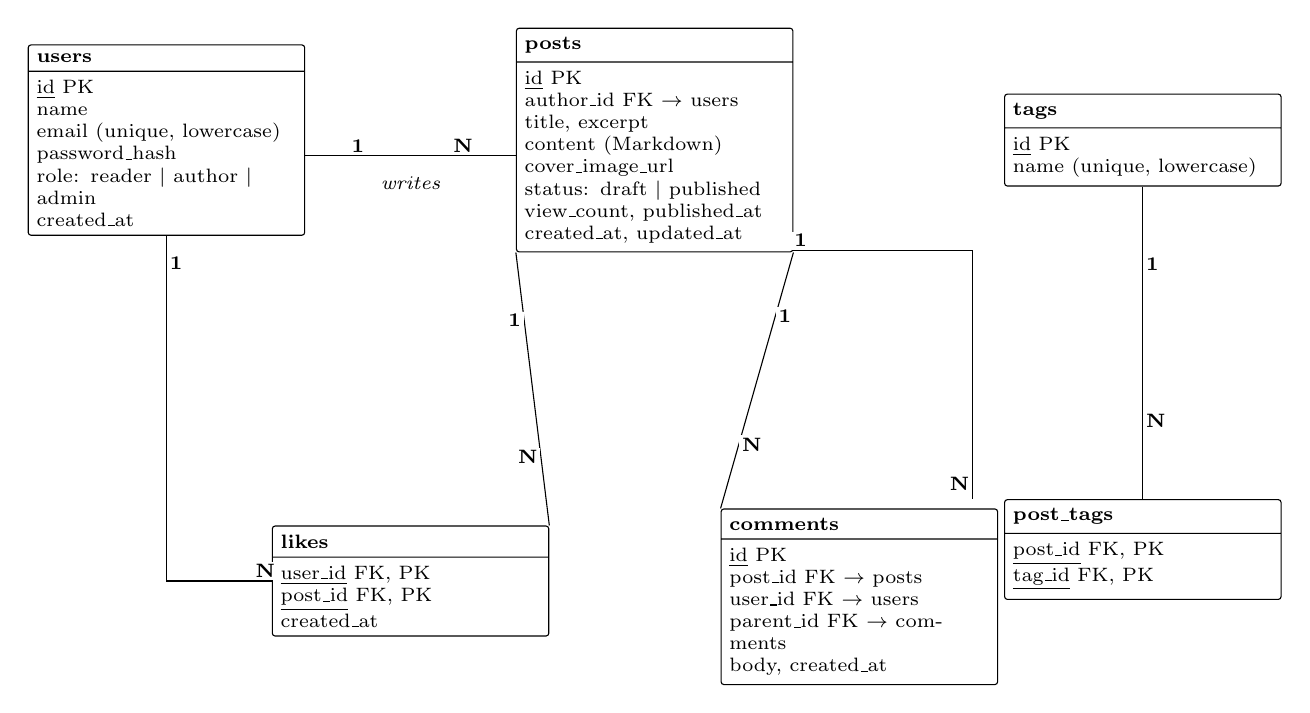
\begin{tikzpicture}[
  ent/.style={draw, rectangle split, rectangle split parts=2, rounded corners=1pt, font=\scriptsize, fill=white, text width=3.3cm, inner sep=3pt},
  card/.style={font=\scriptsize\bfseries, fill=white, inner sep=1pt}
  ]
  \node[ent] (users) at (0,0) {\textbf{users}\nodepart{second}\underline{id} PK\\ name\\ email (unique, lowercase)\\ password\_hash\\ role: reader \textbar{} author \textbar{} admin\\ created\_at};
  \node[ent] (posts) at (6.2,0) {\textbf{posts}\nodepart{second}\underline{id} PK\\ author\_id FK $\rightarrow$ users\\ title, excerpt\\ content (Markdown)\\ cover\_image\_url\\ status: draft \textbar{} published\\ view\_count, published\_at\\ created\_at, updated\_at};
  \node[ent] (tags) at (12.4,0) {\textbf{tags}\nodepart{second}\underline{id} PK\\ name (unique, lowercase)};
  \node[ent] (likes) at (3.1,-5.6) {\textbf{likes}\nodepart{second}\underline{user\_id} FK, PK\\ \underline{post\_id} FK, PK\\ created\_at};
  \node[ent] (cm) at (8.8,-5.8) {\textbf{comments}\nodepart{second}\underline{id} PK\\ post\_id FK $\rightarrow$ posts\\ user\_id FK $\rightarrow$ users\\ parent\_id FK $\rightarrow$ comments\\ body, created\_at};
  \node[ent] (pt) at (12.4,-5.2) {\textbf{post\_tags}\nodepart{second}\underline{post\_id} FK, PK\\ \underline{tag\_id} FK, PK};
  % users 1--N posts
  \draw (users.east |- 0,-0.2) -- node[card, near start, above] {1} node[card, near end, above] {N} (posts.west |- 0,-0.2);
  \node[font=\scriptsize\itshape, fill=white, inner sep=1pt] at (3.1,-0.55) {writes};
  % users 1--N likes
  \draw (users.south) |- node[card, pos=0.04, right] {1} node[card, pos=0.97, above] {N} (likes.west);
  % posts 1--N likes
  \draw (posts.south west) -- node[card, near start, left] {1} node[card, near end, left] {N} (likes.north east);
  % posts 1--N comments
  \draw (posts.south east) -- node[card, near start, right] {1} node[card, near end, right] {N} (cm.north west);
  % posts 1--N post_tags, tags 1--N post_tags
  \draw (posts.east |- 0,-1.4) -| node[card, pos=0.02, above] {1} node[card, pos=0.97, left] {N} ([xshift=-4mm]pt.north west);
  \draw (tags.south) -- node[card, near start, right] {1} node[card, near end, right] {N} (pt.north);
\end{tikzpicture}}
\end{center}
\scriptsize{\emph{Not drawn, to keep it readable:} \code{comments.user\_id} also references \code{users} (who wrote it), and \code{comments.parent\_id} points back to another row of \code{comments} (replies, one level only).}\normalsize

\textbf{Constraints doing real work:} \code{likes} primary key $(user\_id, post\_id)$ = one like per user per post; a \code{BEFORE INSERT} trigger on \code{comments} rejects a reply to a reply or a reply on a different post;
\code{ON DELETE CASCADE} removes a post's comments, likes and tags with it; \code{CHECK} constraints limit lengths and force lowercase emails; Row Level Security is enabled with no policies, so Supabase's public REST API cannot read the tables
(our server connects as the database owner, which bypasses it).

\subsection{B5. React component tree and where state lives}
\begin{center}
\adjustbox{max width=\linewidth}{%
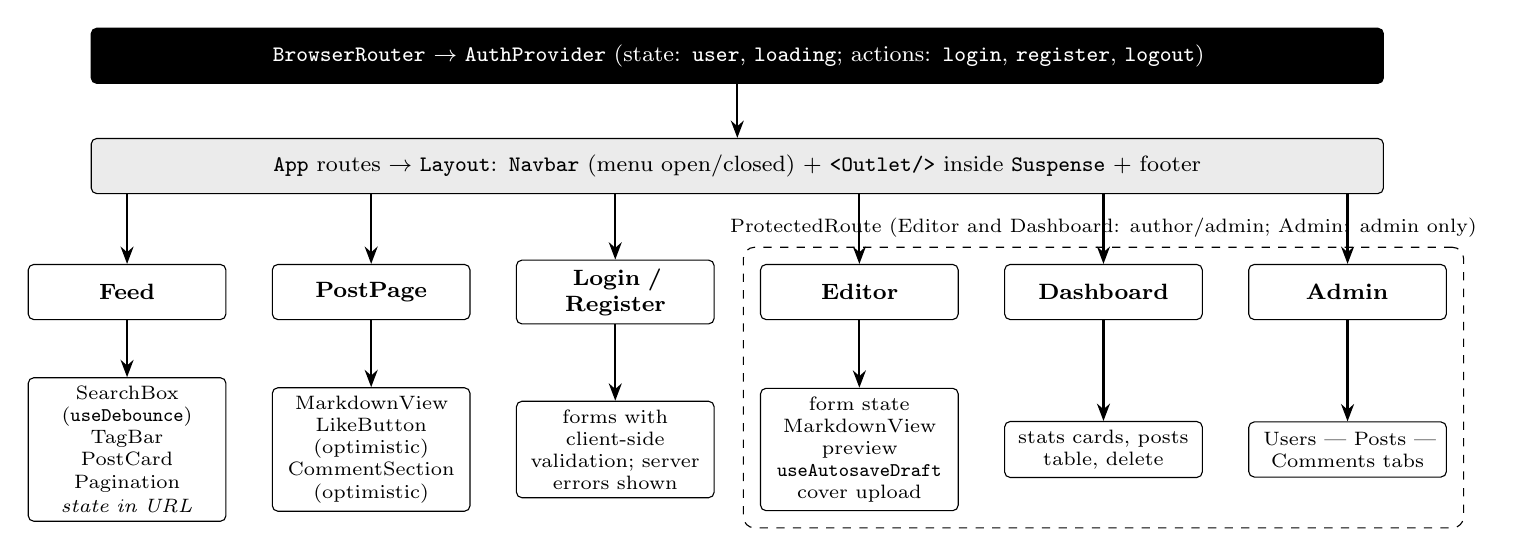
\begin{tikzpicture}[node distance=5mm]
  \node[dark, text width=16.2cm] (root) at (7.75,0) {\code{BrowserRouter} $\rightarrow$ \code{AuthProvider} (state: \code{user}, \code{loading}; actions: \code{login}, \code{register}, \code{logout})};
  \node[soft, text width=16.2cm] (lay) at (7.75,-1.4) {\code{App} routes $\rightarrow$ \code{Layout}: \code{Navbar} (menu open/closed) + \code{<Outlet/>} inside \code{Suspense} + footer};
  \draw[arr] (root) -- (lay);
  \node[box, text width=2.3cm] (p1) at (0,-3.0) {\textbf{Feed}};
  \node[box, text width=2.3cm] (p2) at (3.1,-3.0) {\textbf{PostPage}};
  \node[box, text width=2.3cm] (p3) at (6.2,-3.0) {\textbf{Login / Register}};
  \node[box, text width=2.3cm] (p4) at (9.3,-3.0) {\textbf{Editor}};
  \node[box, text width=2.3cm] (p5) at (12.4,-3.0) {\textbf{Dashboard}};
  \node[box, text width=2.3cm] (p6) at (15.5,-3.0) {\textbf{Admin}};
  \foreach \i in {1,...,6} { \draw[arr] (lay.south -| p\i.north) -- (p\i.north); }
  \node[box, text width=2.3cm, font=\scriptsize] (f1) at (0,-5.0) {SearchBox (\code{useDebounce})\\ TagBar\\ PostCard\\ Pagination\\[1pt] \emph{state in URL}};
  \node[box, text width=2.3cm, font=\scriptsize] (f2) at (3.1,-5.0) {MarkdownView\\ LikeButton (optimistic)\\ CommentSection (optimistic)};
  \node[box, text width=2.3cm, font=\scriptsize] (f3) at (6.2,-5.0) {forms with client-side validation; server errors shown};
  \node[box, text width=2.3cm, font=\scriptsize] (f4) at (9.3,-5.0) {form state\\ MarkdownView preview\\ \code{useAutosaveDraft}\\ cover upload};
  \node[box, text width=2.3cm, font=\scriptsize] (f5) at (12.4,-5.0) {stats cards, posts table, delete};
  \node[box, text width=2.3cm, font=\scriptsize] (f6) at (15.5,-5.0) {Users | Posts | Comments tabs};
  \foreach \i in {1,...,6} { \draw[arr] (p\i.south) -- (f\i.north); }
  \begin{scope}[on background layer]
    \node[zone, fit=(p4) (p5) (p6) (f4) (f5) (f6), label={[font=\scriptsize]above:ProtectedRoute (Editor and Dashboard: author/admin; Admin: admin only)}] {};
  \end{scope}
\end{tikzpicture}}
\end{center}

\subsection{B6. Who can do what}
\begin{tabularx}{\linewidth}{@{}X c c c c@{}}
\toprule
\textbf{Action} & \textbf{Anon} & \textbf{Reader} & \textbf{Author} & \textbf{Admin} \\ \midrule
Read published posts, search, filter by tag & $\bullet$ & $\bullet$ & $\bullet$ & $\bullet$ \\
Like, comment, reply; delete own comment & & $\bullet$ & $\bullet$ & $\bullet$ \\
Create posts, upload cover, dashboard & & & $\bullet$ & $\bullet$ \\
Edit / delete \emph{own} post & & & $\bullet$ & $\bullet$ \\
Edit / delete \emph{any} post, delete \emph{any} comment, see others' drafts, manage roles & & & & $\bullet$ \\
\bottomrule
\end{tabularx}
\emph{Enforced on the server} (\code{requireRole} and ownership checks); hiding buttons in React is only for convenience.

\subsection{B7. API endpoints (base \code{/api}; full examples in \code{openapi.yaml})}
\small
\begin{tabularx}{\linewidth}{@{}>{\ttfamily}l >{\ttfamily}l X@{}}
\toprule
\textbf{Method} & \textbf{Path} & \textbf{Purpose / access} \\ \midrule
GET & /health & Health check (pings database) \\
POST & /auth/register & Create reader/author; returns token \\
POST & /auth/login & Log in; rate limited \\
GET & /auth/me & Current user (token) \\
GET & /posts & Feed: \code{page, limit, q, tag, author} \\
GET & /posts/:id & One post (drafts: owner/admin); counts a view \\
POST & /posts & Create (author, admin) \\
PUT & /posts/:id & Replace (owner, admin) \\
DELETE & /posts/:id & Delete (owner, admin) \\
POST, DELETE & /posts/:id/like & Like / unlike (any logged-in user) \\
GET, POST & /posts/:id/comments & List (nested replies) / add or reply \\
DELETE & /comments/:id & Owner or admin \\
GET & /tags & Tags with published posts \\
GET & /dashboard/posts & My posts with views, likes, comments (author, admin) \\
GET & /admin/users & Admin: users \\
PATCH & /admin/users/:id/role & Admin: change role (not your own) \\
GET & /admin/posts, /admin/comments & Admin: moderation lists \\
POST & /uploads/cover & Image upload $\rightarrow$ resized 1200\,px WebP \\
\bottomrule
\end{tabularx}
\normalsize

\subsection{B8. Status codes we use}
\code{200} OK \quad \code{201} created \quad \code{204} deleted (no body) \quad \code{400} validation failed \quad \code{401} not logged in / bad token \quad \code{403} logged in but not allowed
\quad \code{404} not found (also hides other people's drafts) \quad \code{409} duplicate (email) \quad \code{413} file too large \quad \code{429} too many login attempts \quad \code{500} our bug.

% =====================================================================
\section{Part C --- Quick reference}

\subsection{C1. The SQL that matters (from our routes)}
\begin{lstlisting}[style=sql]
-- Feed: filter + newest first + one page (all values are $1, $2... parameters, never string-glued: no SQL injection)
SELECT p.id, p.title, json_build_object('id', u.id, 'name', u.name) AS author,
       (SELECT count(*)::int FROM likes l WHERE l.post_id = p.id) AS "likeCount"
FROM posts p JOIN users u ON u.id = p.author_id
WHERE p.status = 'published' AND (p.title ILIKE $1 OR p.content ILIKE $1)
ORDER BY p.published_at DESC, p.id DESC
LIMIT $2 OFFSET $3;                        -- OFFSET = (page - 1) * limit

-- Like once: the primary key (user_id, post_id) makes a duplicate impossible; DO NOTHING makes the API idempotent
INSERT INTO likes (user_id, post_id) VALUES ($1, $2) ON CONFLICT DO NOTHING;

-- Tags for a post: create missing tags, then link them (inside a transaction with the post insert)
INSERT INTO tags (name) SELECT unnest($1::text[]) ON CONFLICT (name) DO NOTHING;
INSERT INTO post_tags (post_id, tag_id) SELECT $1, id FROM tags WHERE name = ANY($2::text[]);

-- Dashboard totals per post
SELECT p.id, p.view_count AS views,
       (SELECT count(*)::int FROM likes l WHERE l.post_id = p.id)    AS likes,
       (SELECT count(*)::int FROM comments c WHERE c.post_id = p.id) AS comments
FROM posts p WHERE p.author_id = $1;
\end{lstlisting}
\textbf{Transaction} = all statements succeed or none do (\code{BEGIN} $\ldots$ \code{COMMIT}, \code{ROLLBACK} on error): creating a post and its tags must not leave a post without tags.

\subsection{C2. Environment variables and deployment}
\begin{tabularx}{\linewidth}{@{}>{\ttfamily}l l X@{}}
\toprule
\textbf{Variable} & \textbf{Where} & \textbf{Meaning} \\ \midrule
DATABASE\_URL & Render & Supabase \emph{session pooler} string (IPv4-friendly; the direct string is IPv6-only) \\
DATABASE\_SSL & Render & \code{true} for Supabase \\
JWT\_SECRET & Render & 32+ random characters; never in Git \\
CLIENT\_ORIGIN & Render & Your Vercel URL (CORS) \\
SUPABASE\_URL, SUPABASE\_SERVICE\_ROLE\_KEY, SUPABASE\_BUCKET & Render & Image uploads (service-role key = server only) \\
VITE\_API\_URL & Vercel & \code{https://<render-app>.onrender.com/api} \\
\bottomrule
\end{tabularx}

Order: Supabase (run \code{schema.sql}, create public bucket \code{covers}) $\rightarrow$ Render API $\rightarrow$ Vercel client $\rightarrow$ seed once $\rightarrow$ change demo passwords. Free Render servers sleep: open the site 10 minutes before the demo.

\subsection{C3. Git habits that earn marks}
At least \textbf{5 commits per member}, small and described by what changed: \code{add ownership check to PUT /posts/:id}, not \code{update}. One branch per feature (\code{feat/comments}), merge by pull request, never commit \code{.env} or keys.
Tag the final commit: \code{git tag final-submission \&\& git push --tags}.

\subsection{C4. References}
\begin{itemize}
  \item React: \url{https://react.dev/learn} \quad (Render and Commit: \url{https://react.dev/learn/render-and-commit}; Preserving and Resetting State: \url{https://react.dev/learn/preserving-and-resetting-state}; Custom Hooks: \url{https://react.dev/learn/reusing-logic-with-custom-hooks}; Context: \url{https://react.dev/learn/passing-data-deeply-with-context})
  \item React Router: \url{https://reactrouter.com} \quad Vite: \url{https://vite.dev}
  \item Express: \url{https://expressjs.com} \quad JWT (RFC 7519): \url{https://datatracker.ietf.org/doc/html/rfc7519}
  \item OWASP Password Storage: \url{https://cheatsheetseries.owasp.org/cheatsheets/Password_Storage_Cheat_Sheet.html}
  \item OWASP XSS Prevention: \url{https://cheatsheetseries.owasp.org/cheatsheets/Cross_Site_Scripting_Prevention_Cheat_Sheet.html}
  \item PostgreSQL: \url{https://www.postgresql.org/docs/current/} \quad Supabase connect: \url{https://supabase.com/docs/guides/database/connecting-to-postgres}
  \item Supabase RLS: \url{https://supabase.com/docs/guides/database/postgres/row-level-security} \quad Storage: \url{https://supabase.com/docs/guides/storage}
  \item MDN Fetch: \url{https://developer.mozilla.org/en-US/docs/Web/API/Fetch_API} \quad Render: \url{https://render.com/docs} \quad Vercel: \url{https://vercel.com/docs}
\end{itemize}

\end{document}
